\subsection{Network Flow Monitoring}

Network monitoring is a key component for network management as network administrator derive decisions based on data that results from monitoring activities. By collecting data from network devices, such as switches, routers or clients, the current behaviour of the network is measured. Commonly, this behaviour has to meet some minimum application requirements, which can be summarized by the term Quality of Service (QoS) \cite[406]{tanenbaum2021computer}.


In this context, the most early and vague definition of a network flow was introduced as "a sequence of packets traveling from the source to the destination" \cite{clark1988design}. Here, no further characteristics of a flow are given and it is not clear how one flow is differentiated from another flow. 

In the 1990s, requirement of a more fine grained view on the traffic than interface-level counters queried by Simple Network Management Protocol (SNMP) while at the same time providing significant data reduction compared to packet traces

Now, network flow data has gained a central role in network management operations and research \cite{trammell2011introduction}

since the first standardization approaches in the 1990s durch die Anstrengungen der Internet Engineering Task Force (IETF), a number of dofferent proprietary standards have emerged as each network device vendor implemented its own flow export protocol

In order to improve interoperability in network flow measurement, rufte die IETF die IP Flow Information Export (IPFIX) working group ins Leben. Diese Arbeitsgruppe definierte den gleichnamigen standard IPFIX (RFC 5101), welche den Begriff Network Flow wie folgt definiert.

A network flow is an aggregation of all network packets that pass an observation point of a network during a certain time interval and share a set of common properties. These properties are defined as the result of applying a function to the value of
\begin{enumerate}
    \item one or more packet, transport or application header fields,
    \item one ore more characteristics of the packet itself,
    \item one or more fields derived from packet treatment.
\end{enumerate}

This definition is loose enough to cover the range from a Flow containing all packets observed at a network interface to a flow that consists only of a single packet between two application. At the same time. Note, that the definition of the set of properties is also less strict than the conventional definition of the five-tuple consisting of source IP address, source port, destination IP address, destination port and protocol \cite{rfc5101}

In general, network flows can appear either as unidirectional flow, which aggregates all packets from host A to host B (or vice versa), or as bidirectional format, that aggregates all packets regardless of direction. Depending on which flow format and flow exporter is used, additional information, e.g. statistical calculations on bytes per second, can be obtained. Common formats for network flows are NetFlow \cite{rfc3954}, IPFIX \cite{rfc5101}, OpenFlow \cite{mck_2008} or sFlow \cite{pha_2004}.


\begin{figure}[t]
    \centering
    \documentclass[tikz]{standalone}
\usetikzlibrary{positioning, arrows.meta}
\begin{document}
    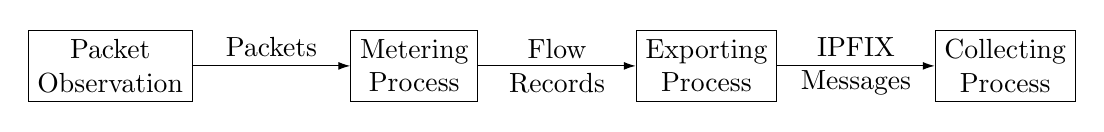
\begin{tikzpicture}[
        arrow/.style =  {-{Latex[length=1.5mm, width=1.0mm]},align=flush center}% 
    ]
        \node[draw, black, align=center] (capture) {Packet \\ Observation};
        \node[draw, black, right=2cm of capture, align=center] (metering) {Metering \\ Process};
        \node[draw, black, right=2cm of metering, align=center] (exporting) {Exporting \\ Process};
        \node[draw, black, right=2cm of exporting, align=center] (collecting) {Collecting \\ Process};

        \draw[arrow] (capture) -- (metering) node[midway,above] {Packets};
        \draw[arrow] (metering) -- (exporting) node[midway, align=center] {Flow \\ Records};
        \draw[arrow] (exporting) -- (collecting) node[midway, align=center] {IPFIX \\ Messages};
    \end{tikzpicture}
\end{document}
    \caption{test}
    \label{fig:flow-export}
\end{figure}


Systems that generate flow data and extract additional information are called flow exporters. Generally, flow exporters are part of a flow monitoring architecture \cite{hof_2014}, which describes four different processes:

\begin{description}
    \item[Packet Observation] Packet observation is done on interfaces of packet forwarding devices by capturing network packets and executing specific preprocessing steps like timestamping and truncation.
    \item[Flow Metering] Flow metering describes the aggregation of packets into flows. There, a set of functions, including packet header capturing, timestamping, sampling and classifying. Furthermore, flow records are maintained, which may include creating, deleting or udpating records, or computing statistical flow features. 
    \item[Exporting] Flow records are placed in a datagram of the deployed export protocol and sends them to one or more collecting processes; encapsulated at the transport layer
    \item[Data Collection] The data collection process is responsible for the reception, storage and preprocessing of flow records, produced by the preceding step.
    \item[Data Analysis] Finally, the collected data is analyzed. This can be done, for example, in the context of \acrshort{ids} or traffic profiling.
\end{description}

Since flow exporters rely on packet header fields and ignore packet payloads, many advantages arise. For example, aggregation results in significant data reduction, which is why an analysis of network flows is scalable and also applicable for high-speed networks \cite{hof_2014}. In addition, discarding the payload results in a better compliance with data retention laws and privacy policies.

The data that is used for network intrusion detection occurs typically in two different levels of granularity. That is network-packet-based data or network-flow-based data. A \acrfull{dpi} approach, that involves the analysis of the payload of network-packet-based data comes along with some drawbacks. For example, \acrshort{dpi} requires highly complex and expensive infrastructure for storage and analysis of the data \cite{hof_2014}, which makes it not feasible for most intrusion detection setups. Therefore, a \acrshort{nids} usually relies on the analysis of network-flows.

% Full packet capturing too much traffic
% notion of network flows is a solution
% what is network flows
% standards (IETF, IPFIX, NetFlow)

% main stages of flow exporting

% benefits: weite Unterstützung, macht QoS skalierbar und günstig, auch gut für security
% which features to extract for NIDS?
% check flow-based IDS works
